\section{Fjernbetjening}

For at øge sikkerheden i forbindelse med flyvning er det besluttet at købe en fjernbetjening til dronen. Fjernbetjeningen skal kunne bruges til at deaktivere den autonome del af dronen og vil udelukkende blive brugt i tilfælde af dronen fejler. 

For at finde den bedst egnede fjernbetjening blev fjernbetjeningen valgt efter følgende kriterier:

\begin{itemize}
	\item Antal kanaler.
	\item Pris.
	\item Rækkevidde.
\end{itemize}

Som udgangspunkt skal fjernbetjeningen minimum have 4 kanaler, disse skal bruges til pitch, roll, throtte og yaw. Udover de 4 kanaler, ønskes yderligere en kanal. Denne kanal skal bruges til at tilkoble/afbryde den autonome del af dronen. Dette betyder at der ønskes en fjernbetjening med minimum 5 kanaler, helst fordelt som vist på figur~\ref{fig:fjernbetjening} 

\begin{figure}[H]
\centering
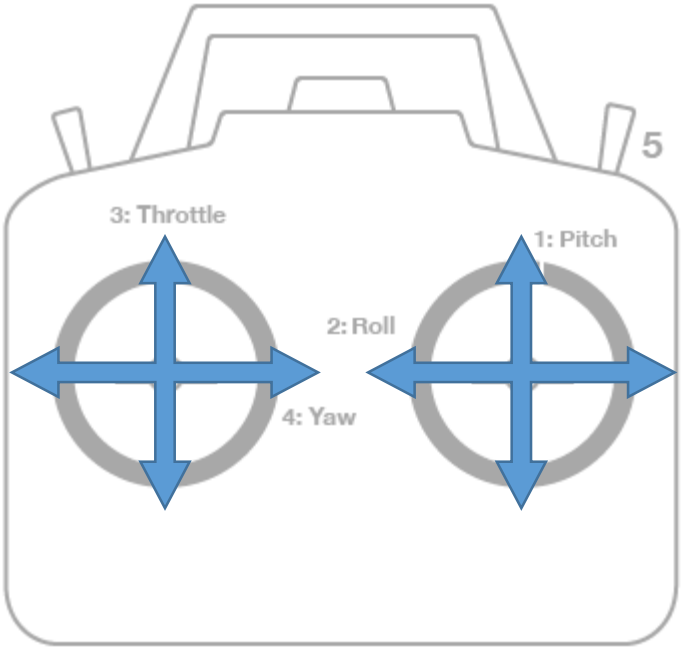
\includegraphics[width=0.5\textwidth]{Billeder/Fjernbetjening}
\caption{Fjernbetjening}
\label{fig:fjernbetjening}
\end{figure}

Fjernbetjeningen har ikke den største funktionalitet i systemet, derfor ønskes det at finde en billig løsning. Da dronen skal flyve autonomt over større områder er det også nødvendigt med en stor rækkevidde på fjernbetjeningen. Baseret på erfaringer fra andre brugere, blev det besluttet at købe en Spektrum DX5e, en 5 kanals fjernbetjening.